\section{Hard- und Software - HS}
\textit{Autor: Hannes Sprafke}

Das folgende Kapitel bezieht sich auf den Teil des Informationsmanagements, den 
Wollnik und Krzmar als Ebene der Informations- und Kommunikationsinfrastruktur 
bezeichnen (vgl. Kapitel \ref{chapter_grundlagen_INM}) Zur Integration eines hochschulweiten 
Informationsmanagements können bezüglich der Hard- und Software mehrere Ansätze 
gefahren werden.

Zum einen kann eine ganzheitliche integrierte Lösung verwendet werden. Die Universität 
Hamburg hat einen vollständigen Neuanfang bezüglich der Campussoftware gewagt mit 
der integrierten Gesamtlösung „CampusNet“ der Datenlotsen Informationssysteme GmbH. 
Die Entscheidung dazu resultierte aus der Zusammenlegung mehrerer Fachbereiche mit 
sehr unterschiedlichen Teillösungen zu einzelnen Fakultäten. Die verschiedenen Teillösungen 
waren größtenteils inkompatibel oder aufgrund von Eigenentwicklung schwer 
wartbar.\footcite[Vgl.][38]{dini_webportale_2007}

Laut Günter Müller, Leiter des Rechenzentrums der Hochschule Emden/Leer, existieren 
an besagter Hochschule derart verschiedene Teillösungen nicht. Auch würden sich derzeit
Eigenentwicklungen bewusst auf vernachlässigbare Systeme beschränken. 
Software würde grundsätzlich für die gesamte Hochschule 
eingesetzt.\footcite{gunter_muller_interview}

Der Einsatz einer integrierten Gesamtlösung zur Beseitigung von Inkompatibilitäten und 
schwer wartbaren Eigenentwicklungen kann somit keine Argumentationsgrundlage sein.
Des Weiteren reicht die in dieser Ausarbeitung getätigte Analyse des Ist-Zustands und 
der Anforderungen nicht aus, um einen vollständigen Anforderungskatalog zu bilden, 
auf dessen Grundlage eine integrierte Gesamtlösung gefunden werden kann.

Stattdessen wird auf eine flexible Lösung gesetzt, welche den Einsatz einzelner 
Fachanwendungen zur Lösung bestimmter Probleme vorsieht. Personelle und 
finanzielle Ressourcen sind dadurch flexibler einsetzbar, auf veränderte Anforderungen 
an eine Lösung kann flexibler reagiert werden und die Abhängigkeit von einem 
Anbieter für alle Anwendungen wird aufgelöst.

Dies ermöglicht eine schrittweise Migration in Form einzelner Projekte. 
Mögliche Strategien dafür werden in Abschnitt \ref{section_migrationskonzepte} näher erläutert. 

\subsection{Kernanforderungen}
Bei Core-Systemen wird weiterhin auf Appliance Lösungen gesetzt. Das minimiert 
Fehlerpotenzial und den operativen Betrieb. \footcite{gunter_muller_interview}

Softwaresysteme laufen auf virtuellen Maschinen. Die bessere Hardwareauslastung 
und Möglichkeit der automatisierten Administration kann finanzielle und 
personelle Ressourcen sparen.\footcite[Vgl.][198]{baun_servervirtualisierung_2009}
Die Systeme sind somit weniger abhängig von der Hardware, was dessen Austausch 
erleichtert. Netzwerkanbindung, Rechenleistung und Speicherkapazität sind somit 
flexibler an sich verändernde Anforderungen anpassbar.

Die eingesetzte Software soll in die Systemlandschaft integrierbar, lösungsorientiert und 
möglichst barrierefrei sein. Um weiterhin verschiedene Teillösungen und Eigenentwicklungen 
zu vermeiden, sollte bei neu einzuführenden Systemen immer geprüft werden, ob bereits 
eine brauchbare Lösung am Markt exisitert.

Da auch das Übertragungsmedium entscheidend zur Erfüllung 
von Informationsbedarfen ist, wie in Abschnitt \ref{subsection_koordination_informationslogistik} 
näher erläutert wurde, soll der Zugang zu Informationen möglichst unabhängig von 
Client-seitig eingesetzten Systemen sein bzw. Unterstützung für möglichst viele 
Zugriffsarten bieten. Diese Freiheit in der Wahl des Mediums unterstützt den Ansatz der 
Freiheit in Forschung und Lehre.

Eine Client-seitige Systemunabhängigkeit kann durch Webanwendungen im Sinne des 
Ansatzes Software as a Service (SaaS) erreicht werden. Um möglichst alle gängigen Browser 
und Endgeräte zu unterstützen, sollten die Anwendungen den Standards des World Wide 
Web Consortiums (W3C) und, soweit möglich, dem Ansatz responsive design gerecht werden. 
Dadurch kann auch dem Trend bring your own device Rechnung getragen werden, wie in 
Abschnitt \ref{netzinfrastruktur_consumerization_und_byod} näher erläutert wurde.

\subsection{Bereichsübergreifende Basissysteme}
Auch wenn eine Hochschule bestimmte Besonderheiten aufweist - vgl. Abschnitt \ref{anwendung_des_inm_auf_hs} - 
fallen dort informationstechnologische Aufgaben an, für die eine zentrale IT-gestützte 
Lösung geschaffen werden kann. Das verringert redundante Daten und Systeme, sowie 
administrative Aufwände. Im folgenden werden Lösungen für einzelne Aspekte des 
Informationsmanagements aus IT-Sicht vorgestellt, die in allen Aufgabenbereichen von 
Hochschulen genutzt werden können. Weiterhin dienen die Lösungen teilweise als Grundlage 
für spezialisierte Systeme oder ermöglichen hilfreiche Erweiterungen dieser.

\subsubsection{Identity Management}
Um die Anzahl an verschiedenen Accounts zu minimieren, sollten die Benutzer zentral gepflegt werden. 
Dies kann in einem Verzeichnisdienst, wie dem bereits eingeführten Active Directory\footcite{gunter_muller_interview}
geschehen. Die Authentifizierung für ein System findet dann nicht am jeweiligen System selbst statt, sondern 
geschieht mit Hilfe des Verzeichnisdienstes. Vorteil ist, dass die Benutzenden sich nur einen Anmeldenamen 
zzgl. Kennwort merken müssen, um sich an den verschiedenen Systemen anzumelden. Weiterhin gilt eine 
Aktualisierung von Informationen global, wodurch Inkonsistenzen aufgelöst werden.

Davon ausgenommen dürfen Systeme sein, deren spezielle Sicherheitsanforderungen nicht mit diesem Konzept 
vereinbar wären. Auch muss die Authentifizierung gesichert geschehen und eine regelmäßige Kennwortänderung 
forciert werden. Auf bestehende Sicherheitsaspekte wurde in Abschnitt \ref{subsection_sicherheitsaspekte} bereits 
eingegangen.

Zuzüglich zum zentralen Verzeichnisdienst ist auch ein SingleSignOn Mechanismus 
empfehlenswert\footnote{siehe Abschnitt \ref{subsubsection_identitatsmanagement}}, 
wie es an der Universität Augsburg durch das System Webauth umgesetzt ist.\footcite[Vgl.][206]{digicampus_2009}

Die an der Hochschule Emden/Leer eingesetzten Websysteme sollen, soweit möglich, vollständig auf SSO umgestellt werden, um dem Benutzer eine möglichst integrierte Landschaft zu bieten. Dies gilt dann auch für einzuführende Systeme. Weiterhin sollte jedes System aus Sicherheitsgründen insofern angepasst werden, dass auch ein SingleSignOff möglich ist.\footcite[Vgl.][150]{kloetgen_2012} Diese zentrale Abmeldung soll gewährleisten, dass die Benutzenden auf allen Systemen, auf denen sie sich bewegt haben, mit einem Klick abgemeldet sind. Der Diebstahl von Websessions bzw. die Fremdnutzung durch Benutzer, die einen Computer anschließend nutzen, kann damit vermieden werden.

Die meisten Systeme bieten eine Benutzerdatenpflege durch den Benutzer selbst an. Diese muss auf den einzelnen Systemen ausgeschaltet sein. Die Benutzenden sollten dennoch die Möglichkeit haben ihre Daten eigenständig zu ändern, allerdings ausschließlich über ein zentrales Formular. So wird ein konsistenter Datenbestand gesichert. Insofern die Informationen in anderen Systemen benötigt werden, müssen diese vom zentralen System wiederkehrend angefordert oder, wenn die Daten im System persistiert sein müssen, automatisiert und über gesicherte Verbindungen verteilt werden.

Ein weiterer Vorteil zentraler Benutzerdaten ist, dass diese zentral ausgewertet werden können. Informationen über Personen können mit Informationen anderer Art aus anderen Systemen angereicht werden um diese weiterzuverwenden. So können automatisierte Reports über Forschungsprojekte erstellt werden, Expertisen zu bestimmten Themen identifiziert werden oder Verknüpfungen von Personen zu verwaltungstechnischen Aufgaben bereitgestellt werden, wie zum Beispiel die Exmatrikulation. Die Umsetzung ist dabei individuell an die Gegebenheiten und Informationsbedarfe der Hochschule anzupassen. Aus diesem Grund wird die technische Lösung eine Individuallösung werden. Diese Individuallösung sollte ein Teil Campus Portals werden, auf das in Abschnitt \ref{subsubsection_campus_portal} eingegangen wird. 

\subsubsection{Geschäftsprozesse}
+Trotz der Freiheit in Forschung und Lehre gibt es an Hochschulen Geschäftsprozesse, die in der Regel immer gleich ablaufen. Bei verstärkter Prozessorientierung werden außerdem vermehrt solche Prozesse entstehen. Ein häufiges Problem bei Geschäftsprozessen ist, dass Personen unterschiedlichster Bereiche involviert sind und die Prozesse häufig nicht transparent genug sind.\footcite[Vgl.][12]{becker_prozesse_2010}

Hier empfiehlt sich der Einsatz von Business Process Management (BPM). BPM dient der Identifizierung, Dokumentation und Verbesserung von Prozessen. Die allgemeine Herangehensweise ist dabei folgende. Nach dem Identifizieren möglicher Prozesse werden diese modelliert, konkretisiert und digitalisiert. Tool unterstützen beim Durchlaufen der digitalisierten Prozesse. Der Verbesserungsprozess, sprich die Anpassung der Prozesse, findet kontinuierlich statt.

Die Modellierung der Prozesse im ersten Schritt sollte auf abstraktem Niveau stattfinden. Dies erleichtert den Einstieg und macht Verbesserungspotenziale sichtbarer. In der WWU Münster wurde dafür die PICTURE Methode verwendet.\footcite[Vgl.][16]{becker_prozesse_2010} Wichtig ist die Einbeziehung der Prozessbeteiligten. Abschnitt \ref{section_changemanagement} setzt sich mit den Besonderheiten des Change Managements an Hochschulen detaillierter auseinander.

Im zweiten Schritt kann der ggf. angepasste Prozess konkretisiert und in Form des Industriestandards Business Process Model Notation (BPMN) digital notiert werden. Ein Client-Tool zur Erstellung von BPMN ist das Activiti BPMN 2.0 Eclipse Plugin.\footcite{eclipse_bpmn2_modeler}

Mit Hilfe der zentralen Business Process Management (BPM) Platform activiti können die Prozesse aktiv den Workflow verbessern, Konsistenz wahren und zeitliche Ressourcen sparen.  Die Plattform ermöglicht REST Anfragen, wodurch die Prozessinformationen auch in andere Applikation integriert werden können. Der Activiti Explorer ermöglicht den voll funktionalen Zugriff via Weboberfläche. Somit wird der Kernanforderung SaaS Rechnung getragen. Weiterhin ist Activiti Open Source und somit ausbau- und anpassungsfähig.\footcite{activiti_website}

Durch activiti wird es möglich sein die Automatisierung von einzelnen Prozessen Stück für Stück voranzutreiben indem manuelle Aufgaben gegen Automatismen ersetzt werden. Einzelne Teile des Workflows können dann automatisiert Scripte starten, E-Mails verschicken und ähnliches und somit stückweise die manuelle Bearbeitung reduzieren. Durch Definition von Pflichtfeldern für einzelne Prozessschritte können vorab benötigte Informationen festgelegt werden, sodass Nachfragen vermieden werden.

\subsubsection{Content Management}
Um den wachsenden Anforderungen in Bezug auf Content Management genüge zu tun, wurde an der WWU Münster das Enterprise Content Management System Alfresco eingeführt. Auch an einer kleinen Hochschule kann ein solches System eingesetzt werden. Alfresco bietet diverse Vorteile. Die für dieses Konzept Relevanten werden hier kurz aufgelistet:\footcite[Vgl.][47 ff.]{kloetgen_2012}

\begin{itemize}
	\item Unterstützung für mobile Endgeräte
	\item Anpassungs- und ausbaufähig
	\item diverse Zugriffsmöglichkeiten zur Nutzung innerhalb bekannter Standardanwendungen
	\item Publikation in sozialen Netzwerken
	\item Unterstützung verschiedener Standardschnittstellen
	\item Activiti Workflow Engine
	\item Metadaten
\end{itemize}

Alfresco bietet damit die ideale Grundlage verschiedenste Informationen zu verwalten, sowie die Unterstützung des vollständigen Dokumenten-Lifecycles: von der Erstellung über die Bereitstellung bis zur Archivierung.

Die Art des Zugriffs auf Dokumente ist dynamisch dank der Unterstützung zahlreicher Standards. Somit kann eine Integration des Zugriffs auf Dokumente, angepasst an die jeweiligen Anforderungen eines benutzenden Systems, geschehen. Ein Dokument, welches an verschiedenen Orten auf verschiedene Arten bereitgestellt werden soll, kann dank Alfresco zentral aktualisiert werden. Die zugreifenden Systeme erhalten immer genau den Lifecyle-Version des Dokuments, der für sie vorgesehen ist.

Dank der integrierten Versionierung entfällt außerdem der aufwendige Wiederherstellungsprozess bei Dateisystem-basierten Sicherungen.

Durch die Möglichkeit Metadaten anzugeben, wird der Weg für eine brauchbare Dokumentensuche geebnet. 
Diese kann in die integrierte Gesamtsuche einbezogen werden.\footnote{siehe Abschnitt \ref{subsubsection_integrierte_gesamtsuche}}

\subsection{Spezialsysteme}
Unter Spezialsystemen sind hier Softwarelösungen zu verstehen, die bei speziellen Aufgaben im Hochschulalltag unterstützen sollen, wie zum Beispiel die Bereitstellung von Lehrmaterial oder die Evaluation von Kursen.

\subsubsection{Lernplattform}
Die Hochschule Emden/Leer setzt bereits erfolgreich und in allen Fachbereichen das System moodle als Lernplatform ein.\footcite{gunter_muller_interview} 
Die Nutzung der Funktionen variiert dabei jedoch zwischen den einzelnen Fachbereichen.\footnote{siehe Abschnitt \ref{subsection_e-learning}}
Solange moodle die Anforderungen der Hochschule an eine Lernplattform erfüllt, besteht kein Grund das System auszutauschen.

Neben den bereits genutzten Standardfunktionen ist moodle ausbaufähig.

Beim Aufruf von moodle soll die Authentifizierung durch einen SSO Mechanismus geschehen. Für das Lernraumsystem moodle gibt es bereits ein SSO Plugin.\footcite{macklin_moodle_sso_plugin} Integriert werden sollte, wie in Kapitel 6.3.2.1 erläutert, dann auch ein Single-Sign-Off Mechanismus.

Statt der Stammdatenänderung via moodle wird der entsprechende Menüpunkt ausgeblendet werden bzw. die Benutzenden auf ein zentrales Formular weiterleiten, um persönliche Informationen zentral und damit konsistent zu halten.

Die in den Kursen zur Verfügung gestellten Dateien jeglicher Art werden in Alfresco gepflegt und von moodle angebunden. Die entsprechenden Schnittstellen und Plugins existieren bereits auf dem Markt und müssen somit nicht neu entwickelt werden.

Vorteil der Integration von Alfresco in moodle ist, dass damit die Vorteile Alfrescos zur Dokumentenverwaltung genutzt werden können. In moodle kann dann eine bestimmte Version oder die jeweils aktuellste referenziert werden. Bei den Dokumenten kann es sich um Textdokumente, Audio- oder auch Videodateien handeln. Durch Alfrescos Unterstützung für mobile Endgeräte wird den Zugreifenden die Möglichkeit gegeben, ein Dokument auf verschiedensten Endgeräten anzuzeigen bzw. wiederzugeben. Außerdem können dank Alfresco diese Dokumente nicht nur innerhalb von moodle via Weboberfläche aufgerufen werden, sondern über verschiedene Medien angebunden werden, zum Beispiel via Filesystem in Form eines Netzwerk-Shares. 
Damit wird eine Freiheit in der Wahl des Übertragungsmedium gewährleistet.\footnote{siehe Abschnitt\ref{subsection_koordination_informationslogistik}}

Ein mögliches Migrationskonzept wird in Abschnitt \ref{subsubsection_changemanagement_alfresco} erläutert.

\subsubsection{Publikationen}
Um Wissenschaftler bei der Publikation von Zeitschriften zu unterstützen, kann die Plattform Open Journal System (OJS) eingesetzt werden, wie es auch in der WWU Münster getan wird. Es bietet die Möglichkeit elektronische Zeitschriften zu verwalten und den gesamten Publikationsworkflow abzubilden.\footcite[Vgl.][48]{vogl_fortschritte_2012}

Zusätzlich sollte auch ein Workflow in activiti implementiert werden, der bei der Publikation unterstützt. So können wichtige Metadaten aufgenommen und an relevante Systeme weitergegeben werden. Ändern sich Systeme oder kommen neue hinzu, müssen sich Wissenschaftler nicht umgewöhnen, sondern nutzen weiterhin den in activiti hinterlegten, für die neuen Systeme jedoch angepassten, Prozess. Dadurch besteht auch die Möglichkeit ein publiziertes Dokument zusätzlich in Alfresco abzulegen, wenn ein Anwendungsfall dies benötigt.

OJS bietet die Möglichkeit der Authentifizierung via Single Sign On. Dies geschieht via Shibboleth.\footcite{ojs_setup_sso} 
Neben der Konfiguration von SSO sollte auch hier wieder den Benutzenden die Möglichkeit des Single-Sign-Offs gegeben werden.

\subsubsection{Evaluation}
Wie auch die Universität Münster\footcite{evasys_muenster} und die TU Dortmund\footcite{evasys_dortmund} setzt die Hochschule Emden/Leer bereits die Software EvaSys zu Evaluationszwecken ein.\footcite{gunter_muller_interview} Sie ist webbasiert und entspricht damit dem SaaS Prinzip.
Seit Version 5 unterstützt EvaSys auch die SSO Authentifizierung\footcite{evasys_sso}, welche auch an der Hochschule Emden/Leer eingesetzt werden soll.

\subsubsection{Campus Portal}
\label{subsubsection_campus_portal}
Ein Campus Portal dient als zentrale Anlaufstelle für alle Hochschulangehörigen und ist ein personalisiertes Webportal. Es soll die Verwaltung persönlicher Daten ermöglichen, eine Übersicht über informationstechnische Funktionen, inklusive Weiterleitung zum entsprechenden System, integrieren, sowie aktuell relevante personalisierte Informationen in Form einer Agenda anzeigen. Das Campus Portal dient also als Startpunkt.

Hinter den informationstechnischen Funktionen stecken alle Werkzeuge und Spezialsysteme, die einem bestimmten Zweck dienen. Auf einige davon wurde in den vorhergehenden Unterkapiteln bereits eingegangen. Bei der Integration solcher Systeme werden nun die anfangs genannten Kernanforderungen an solche Systeme, nämlich integrierbar und systemunabhängig (SaaS) zu sein, deutlich.

Ein solches Campus Portal ist vor allem der Informationsübersicht dienlich. Durch personalisierte und dynamisch generierte Inhalte gewinnen die Benutzenden einen Überblick über die Informationen\footcite[Vgl.][24]{dini_webportale_2007}, die sonst ausschließlich in den verschiedenen Systemen verteilt sind. Der Aufbau eines Campus Portals und die Integration der Spezialsysteme kann schrittweise erfolgen, sollte jedoch zur Akzeptanzgewinnung bei Veröffentlichung eine gewisse Menge externer Systeme integrieren.\footcite[Vgl.][17 f.]{dini_webportale_2007} Die Universität Karlsruhe hat im ersten Schritt das Veranstaltungsmanagement und die Prüfungsverwaltung der Software-Systeme der HIS GmbH in das Portal integriert.\footcite[Vgl.][40 f.]{dini_webportale_2007}

Aufgrund der Individualität der fachlichen und technischen Anforderungen wird es an der Hochschule Emden/Leer wahrscheinlich auf eine Individuallösung hinauslaufen.\footcite[Vgl.][21]{dini_webportale_2007} Vorsicht! Die Aufwände für die Umsetzung eines Campus Portals sind in der Kosten- und Zeitschätzung für das Redesign der Hochschul-Webseite nicht integriert.

Orientiert am Anforderungskatalog der WWU Münster an ein solches Portal und unter der Voraussetzung, dass die in diesem Konzept genannten Systeme 
umgesetzt werden, kann ein zukünftiges CampusPortal der Hochschule Emden/Leer folgende Informationen konsolidieren:\footcite[Vgl.][158 ff.]{vogl_fortschritte_2012}

\begin{itemize}
	\item Kalender
	\begin{itemize}
		\item Abonnement-Prinzip
		\item inklusive Detailinformationen, zum Beispiel Kontoinformationen für Rückmeldegebühren
		\item Agenda aus moodle
	\end{itemize}
	\item Referenz zu gewählten Kursen (moodle)
	\item Referenz zum E-Mail-Portal (Outlook Web App)
	\item Suchmaschine
	\item offene Tasks im BPM System
	\item Start möglicher Tasks im BPM System (zum Beispiel Workflow für die Publikation)
	\item offene Evaluationen
\end{itemize}

Neben den in diesem Konzept genannten Systemen, könnten weitere Spezialsysteme in das Campus Portal integriert werden, sofern diese entsprechende Schnittstellen aufweisen. Der Anforderungskatalog der WWU Münster enthält außerdem:

\begin{itemize}
	\item Stundenplan
	\item Vorlesungsverzeichnis inkl. Details
	\item Leistungsübersicht
	\item Hochschulleben
	\begin{itemize}
		\item Mensapläne
		\item Hochschulsport
		\item Veranstaltungen
	\end{itemize}
	\item Einführung in die Benutzung
\end{itemize}

Alternativ zur Einführung in die Benutzung kann auch das Konzept eines Hilfesystems integriert werden, das via Sprechblasen Hilfestellungen oder Erläuterungen anzeigt zur jener Funktionalität, auf der sich der Mauszeiger gerade befindet.\footcite[Vgl.][22]{vogl_bericht_2013}

Die technische Struktur kann analog zu der des Portals myWWU der Universität Münster aufgebaut sein, wie im Folgenden abgebildet.\footcite[Vgl.][165]{vogl_fortschritte_2012}
\begin{figure}[h!]
	\centering
	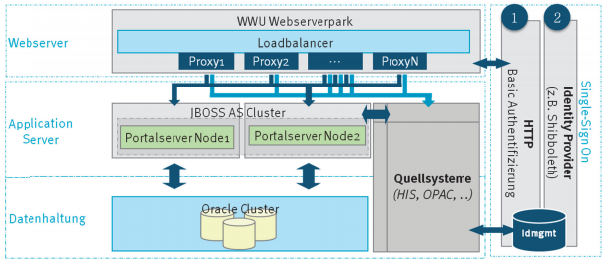
\includegraphics[width=\textwidth]{kapitel/gruppe3/bilder/struktur_mywwu}
	\caption{technische Struktur des Portals myWWU der Universität Münster}
	\label{fig_struktur_mywwu}
\end{figure}
\newpage

\subsubsection{Integrierte Gesamtsuche}
\label{subsubsection_integrierte_gesamtsuche}
Wissenschaftliche Informationen sind häufig in verschiedenen Systemen angesiedelt. Durch die Einführung eines Systems zur integrierten Gesamtsuche würde die Suche an zentraler Stelle ausgeführt. Einzelne Systeme werden von den Suchenden nicht vergessen und die Integration neuer wissenschaftlicher Informationssysteme wird dauerhaft kommuniziert statt einmalig, wie es beispielsweise beim 
Versand einer Info-E-Mail der Fall wäre.

Die WWU Münster nutzt dafür einen „Suchmaschinen-basierte[n] Ansatz auf Basis der Software Primo von der Firma Ex Libris“.\footcite[Vgl.][41]{vogl_fortschritte_2012} Dafür nötig ist eine Normalisierung der Datenformate interner und externer Quellen, welche „insbesondere auf der Detailebene […] aufwändige Anpassungen und Eigenentwicklungen notwendig“ machen.\footcite[Vgl.][42]{vogl_fortschritte_2012}

Quellsysteme, ausgehend von diesem Konzept, können sein:
\begin{itemize}
	\item Alfresco
	\item Identity Management System
	\item ForschungsDB Niedersachsen
	\item moodle
	\item Open Journal System
	\item Hochschulexterne Informationssysteme wie zum Beispiel video2brain
	\item ggf. Bibliothekssuche
\end{itemize}

Wichtig ist neben korrekten und vollständigen Ergebnissen auch die Benutzbarkeit. Bekannte Funktionalitäten aus anderen Suchmaschinen, wie Gruppierungen, sollten integriert sein, wie auch eine übersichtliche und funktionale Benutzeroberfläche.\footcite[Vgl.][43]{vogl_fortschritte_2012}

\subsection{Ausblick bei Integration der Bibliothek}
Auch wenn die Bibliothek in dieser Ausarbeitung ausgenommen ist, muss erwähnt werden, dass bei Informationsmanagement-Projekten anderer Hochschulen und Universitäten auch die Bibliotheken integriert werden. Die über die Bibliothek zur Verfügung gestellten Informationen werden vor allem für Forschung und Lehre genutzt, welches die Kernaufgaben von Hochschulen sind.

Dementsprechend kann die Integration der Bibliothekssuche in die integrierte Gesamtsuche zur Aufwertung der Suchergebnissen beitragen. Um auch nicht digital verfügbare bzw. archivierte Zeitschriften und Bücher integrieren zu können, kann ein Digitalisierungssystem eingeführt werden. Die WWU Münster setzt dafür vor Ort frei verfügbare Scanner zuzüglich der Software scantoweb ein.\footcite[Vgl.][50]{vogl_fortschritte_2012}
